\batchmode
\makeatletter
\def\input@path{{/Users/wesley/git/gwr/writeup/estimation//}}
\makeatother
\documentclass[12pt,english,authoryear,review, 12pt]{elsarticle}\usepackage[]{graphicx}\usepackage[]{color}
%% maxwidth is the original width if it is less than linewidth
%% otherwise use linewidth (to make sure the graphics do not exceed the margin)
\makeatletter
\def\maxwidth{ %
  \ifdim\Gin@nat@width>\linewidth
    \linewidth
  \else
    \Gin@nat@width
  \fi
}
\makeatother

\definecolor{fgcolor}{rgb}{0.345, 0.345, 0.345}
\newcommand{\hlnum}[1]{\textcolor[rgb]{0.686,0.059,0.569}{#1}}%
\newcommand{\hlstr}[1]{\textcolor[rgb]{0.192,0.494,0.8}{#1}}%
\newcommand{\hlcom}[1]{\textcolor[rgb]{0.678,0.584,0.686}{\textit{#1}}}%
\newcommand{\hlopt}[1]{\textcolor[rgb]{0,0,0}{#1}}%
\newcommand{\hlstd}[1]{\textcolor[rgb]{0.345,0.345,0.345}{#1}}%
\newcommand{\hlkwa}[1]{\textcolor[rgb]{0.161,0.373,0.58}{\textbf{#1}}}%
\newcommand{\hlkwb}[1]{\textcolor[rgb]{0.69,0.353,0.396}{#1}}%
\newcommand{\hlkwc}[1]{\textcolor[rgb]{0.333,0.667,0.333}{#1}}%
\newcommand{\hlkwd}[1]{\textcolor[rgb]{0.737,0.353,0.396}{\textbf{#1}}}%

\usepackage{framed}
\makeatletter
\newenvironment{kframe}{%
 \def\at@end@of@kframe{}%
 \ifinner\ifhmode%
  \def\at@end@of@kframe{\end{minipage}}%
  \begin{minipage}{\columnwidth}%
 \fi\fi%
 \def\FrameCommand##1{\hskip\@totalleftmargin \hskip-\fboxsep
 \colorbox{shadecolor}{##1}\hskip-\fboxsep
     % There is no \\@totalrightmargin, so:
     \hskip-\linewidth \hskip-\@totalleftmargin \hskip\columnwidth}%
 \MakeFramed {\advance\hsize-\width
   \@totalleftmargin\z@ \linewidth\hsize
   \@setminipage}}%
 {\par\unskip\endMakeFramed%
 \at@end@of@kframe}
\makeatother

\definecolor{shadecolor}{rgb}{.97, .97, .97}
\definecolor{messagecolor}{rgb}{0, 0, 0}
\definecolor{warningcolor}{rgb}{1, 0, 1}
\definecolor{errorcolor}{rgb}{1, 0, 0}
\newenvironment{knitrout}{}{} % an empty environment to be redefined in TeX

\usepackage{alltt}
\usepackage[T1]{fontenc}
\usepackage[latin9]{inputenc}
\setlength{\parskip}{\bigskipamount}
\setlength{\parindent}{0pt}
\usepackage{array}
\usepackage{verbatim}
\usepackage{bm}
\usepackage{multirow}
\usepackage{amsthm}
\usepackage{amsmath}
\usepackage{amssymb}
\usepackage{graphicx}
\usepackage{setspace}
\doublespacing

\makeatletter

%%%%%%%%%%%%%%%%%%%%%%%%%%%%%% LyX specific LaTeX commands.
%% Because html converters don't know tabularnewline
\providecommand{\tabularnewline}{\\}

%%%%%%%%%%%%%%%%%%%%%%%%%%%%%% Textclass specific LaTeX commands.
\usepackage[natbibapa]{apacite}
\theoremstyle{plain}
\newtheorem{thm}{\protect\theoremname}

%%%%%%%%%%%%%%%%%%%%%%%%%%%%%% User specified LaTeX commands.
\setlength{\topmargin}{0in}
\setlength{\oddsidemargin}{0in}
\setlength{\evensidemargin}{0in}

\makeatother

\usepackage{babel}
\providecommand{\theoremname}{Theorem}
\IfFileExists{upquote.sty}{\usepackage{upquote}}{}
\begin{document}

\title{Local Adaptive Grouped Regularization and its Oracle Properties}


\author{Wesley Brooks, Jun Zhu, Zudi Lu}


\section{Introduction}

Whereas the coefficients in traditional linear regression are scalar
constants, the coefficients in a varying coefficients regression (VCR)
model are functions - often \emph{smooth} functions - of some effect-modifying
variable \citep{Hastie:1993a,Cleveland-Grosse-1991}.

Current practice for VCR models relies on global model selection to
decide which variables should be included in the model, meaning that
predictors are identified as relevant or irrelevant over the entire
domain. \citet{Antoniadis:2012a} describe a method for globally selecting
the relevant predictors in a VCR model where the coefficient functions
are estimated with P-splines. \citet{Wang-2008a} show a method for
doing global variable selection in a VCR model where the coefficient
functions are estimated by basis expansion.

Local adaptive grouped regularization (LAGR) is developed here as
a method to select only the locally relevant predictors at any specific
location $\bm{s}$ in the domain $\mathcal{D}$ of a VCR model. The
method of LAGR applies to VCR models where the coefficients are estimated
using locally linear kernel smoothing. Using kernel smoothing for
nonparametric regression is described in detail in \citet*{Fan-Gijbels-1996}.
The extension to estimating VCR models is made by \citet{Fan-Zhang-1999}
for a VCR a univariate effect-modifying variable, and by \citet{Sun-Yan-Zhang-Lu-2014}
for two-dimensional effect-modifying variable and autocorrelation
among the obverved response. These methods minimize the boundary effect
\citep{Hastie:1993b} by estimating the coefficients as local polynomials
of odd degree (usually locally linear).

For linear regression models, the adaptive lasso (AL) produces consistent
estimates of the coefficients and has been shown to have appealing
properties for variable selection which, under suitable conditions,
include the ``oracle'' property of asymptotically including exactly
the correct set of covariates and estimating their coefficients as
well as if the correct covariates were known in advance \citep{Zou-2006}.
For data where the obvserved variables fall into mutually exclusive
groups that are known in advance, the adaptive group lasso has similar
oracle properties to the adaptive lasso while doing selection at the
level of groups rather than individual variables \citep{Yuan-Lin-2006,Wang-Leng-2008}.
The proposed LAGR method uses the adaptive group lasso for local variable
selection and coefficient estimation in a locally linear regression
model. We show that LAGR posesses the oracle properties of asymptotically
selecting exactly the correct local predictors and estimating their
local coefficients as accurately as would be possible if the identity
of the nonzero coefficients for the local model were known in advance.

The remainder of this document is organized as follows. The kernel-based
VCR model is described in Section \ref{sec:vcr}. The proposed LAGR
technique and its oracle properties are presented in Section \ref{sec:lagr-gaussian}.
In Section \ref{sec:simulations}, the performance of the proposed
LAGR technique is evaluated in a simulation study, and in Section
\ref{sec:example} the proposed method is applied to the Boston house
price dataset. Proofs of the theorems appear in Appendix \ref{app:proofs}.


\section{Varying coefficients regression\label{sec:vcr}}


\subsection{Model}

Consider $n$ data points, observed at sampling locations $\bm{s}_{i}=(s_{i,1},\; s_{i,2})^{T}$
for $i=1,\dots,n$, which are distributed in a spatial domain $\mathcal{D}\subset\mathbb{R}^{2}$
according to a density $f(\bm{s})$ with $\bm{s}\in\mathcal{D}$.
For $i=1,\dots,n$, let $y(\bm{s}_{i})$ and $\bm{x}(\bm{s}_{i})$
denote, respectively, the univariate response and the $(p+1)$-variate
vector of covariates measured at location $\bm{s}_{i}$. At each location
$\bm{s}_{i}$, assume that the outcome is related to the covariates
by a linear regression where the coefficients $\bm{\beta}(\bm{s}_{i})$
may be spatially-varying and $\varepsilon(\bm{s}_{i})$ is random
error at location $\bm{s}_{i}$. That is, 
\begin{align}
y(\bm{s}_{i})=\bm{x}(\bm{s}_{i})'\bm{\beta}(\bm{s}_{i})+\varepsilon(\bm{s}_{i}).\label{eq:lm(s)}
\end{align}


Further assume that the error term $\varepsilon(\bm{s}_{i})$ is normally
distributed with zero mean and variance $\sigma^{2}$, and that $\varepsilon(\bm{s}_{i})$,
$i=1,\dots,n$ are independent. That is, 
\begin{align}
\bm{\varepsilon}\overset{iid}{\sim}\mathcal{N}\left(0,\sigma^{2}\right).\label{eq:err}
\end{align}


In the context of nonparametric regression, the boundary-effect bias
can be reduced by local polynomial modeling, usually in the form of
a locally linear model \citep{Fan-Gijbels-1996}. Here, to prepare
for the estimation of locally linear coefficients, we augment the
local design matrix with covariate-by-location interactions in two
dimensions \citep{Wang-2008b}. The augmented local design matrix
at location $\bm{s}_{i}$ is 
\begin{align}
\bm{Z}(\bm{s}_{i})=\left(\bm{X}\:\: L_{i}\bm{X}\:\: M_{i}\bm{X}\right)
\end{align}


where $\bm{X}$ is the unaugmented matrix of covariates, $\bm{L}_{i}=\text{diag}\{s_{i',1}-s_{i,1}\}$
and $\bm{M}_{i}=\text{diag}\{s_{i',2}-s_{i,2}\}$ for $i'=1,\dots,n$.

Now we have that $Y(\bm{s}_{i})=\left\{ \bm{Z}(\bm{s}_{i})\right\} _{i}^{T}\bm{\zeta}(\bm{s}_{i})+\varepsilon(\bm{s}_{i})$,
where $\left\{ \bm{Z}(\bm{s}_{i})\right\} _{i}^{T}$ is the $i$th
row of the matrix $\bm{Z}(\bm{s}_{i})$ as a row vector, and $\bm{\zeta}(\bm{s}_{i})$
is the vector of local coefficients at location $\bm{s}_{i}$, augmented
with the local gradients of the coefficient surfaces in the two spatial
dimensions, indicated by $\nabla_{u}$ and $\nabla_{v}$:

\[
\bm{\zeta}(\bm{s}_{i})=\left(\bm{\beta}(\bm{s}_{i})^{T},\;\nabla_{u}\bm{\beta}(\bm{s}_{i})^{T},\;\nabla_{v}\bm{\beta}(\bm{s}_{i})^{T}\right)^{T}
\]



\subsection{Local Likelihood and Coefficient Estimation}

The total log-likelihood of the observed data is the sum of the log-likelihood
of each individual observation: 
\begin{align}
\ell\left(\bm{\zeta}\right)=-(1/2)\sum_{i=1}^{n}\left[\log{\sigma^{2}}+\sigma^{-2}\left\{ y(\bm{s}_{i})-\bm{z}'(\bm{s}_{i})\bm{\zeta}(\bm{s}_{i})\right\} ^{2}\right].\label{eq:coefficients}
\end{align}


Since there are a total of $n\times3(p+1)+1$ parameters for $n$
observations, the model is not identifiable and it is not possible
to directly maximize the total likelihood. But when the coefficient
functions are smooth, the coefficients at location $\bm{s}$ can approximate
the coefficients within some neighborhood of $\bm{s}$, with the quality
of the approximation declining as the distance from $\bm{s}$ increases.

This intuition is formalized by the local (log-)likelihood, which
is maximized at location $\bm{s}$ to estimate the local coefficients
$\bm{\zeta}(\bm{s})$:

\begin{align}
\ell\left(\bm{\zeta}(\bm{s})\right) & =-(1/2)\sum_{i=1}^{n}K_{h}(\|\bm{s}-\bm{s}_{i}\|)\left[\log{\sigma^{2}}+\sigma^{-2}\left\{ y(\bm{s}_{i})-\bm{z}'(\bm{s}_{i})\bm{\zeta}(\bm{s})\right\} ^{2}\right]\label{eq:local-log-likelihood}
\end{align}


where $h$ is a bandwidth parameter and the $K_{h}(\|\bm{s}-\bm{s}_{i}\|)$
for $i=1,\dots,n$ are local weights from a kernel function. For instance,
the Epanechnikov kernel is defined as \citep{Samiuddin-el-Sayyad-1990}:
\begin{align}
K_{h}(\|\bm{s}_{i}-\bm{s}_{i'}\|) & =h^{-2}K\left(h^{-1}\|\bm{s}_{i}-\bm{s}_{i'}\|\right)\notag\label{eq:epanechnikov}\\
K(x) & =\begin{cases}
(3/4)(1-x^{2}) & \mbox{ if }x<1,\\
0 & \mbox{ if }x\geq1.
\end{cases}
\end{align}


Letting $\bm{W}(\bm{s})=diag\left\{ K_{h}(\|\bm{s}-\bm{s}_{i}\|)\right\} $
be a diagonal matrix of kernel weights, the local likelihood is maximized
by weighted least squares: 
\begin{align}
\mathcal{S}\left\{ \bm{\zeta}(\bm{s})\right\}  & =(1/2)\left\{ \bm{Y}-\bm{Z}(\bm{s})\bm{\zeta}(\bm{s})\right\} ^{T}\bm{W}(\bm{s})\left\{ \bm{Y}-\bm{Z}(\bm{s})\bm{\zeta}(\bm{s})\right\} ^{T}\notag\label{eq:zeta-hat}
\end{align}


Thus, we have

\[
\tilde{\bm{\zeta}}(\bm{s})=\left\{ \bm{Z}^{T}(\bm{s})\bm{W}(\bm{s})\bm{Z}(\bm{s})\right\} ^{-1}\bm{Z}^{T}(\bm{s})\bm{W}(\bm{s})\bm{Y}
\]


Now Theorem 3 of \citet{Sun-Yan-Zhang-Lu-2014} says that, for any
given $\bm{{s}}$

\[
\sqrt{{nh^{2}f(\bm{{s}})}}\left[\hat{\bm{\beta}}(\bm{s})-\bm{\beta}(\bm{s})-(1/2)\kappa_{0}^{-1}\kappa_{2}h^{2}\left\{ \bm{\beta}_{uu}(\bm{s})+\bm{\beta}_{vv}(\bm{s})\right\} \right]\xrightarrow{{D}}N\left(\bm{0},\kappa_{0}^{-2}\nu_{0}\sigma^{2}\Psi^{-1}\right)
\]



\section{Local Variable Selection with LAGR\label{sec:lagr-gaussian}}


\subsection{The LAGR-Penalized Local Likelihood}

Estimating the local coefficients by (\ref{eq:zeta-hat}) relies on
\emph{a priori} variable selection. A new method of penalized regression
to simultaneously select the locally relevant predictors and estimate
the local coefficients. For this purpose, each raw covariate is grouped
with its covariate-by-location interactions. That is, $\bm{\zeta}_{j}(\bm{s})=\left(\beta_{j}(\bm{s})\;\;\;\nabla_{u}\beta_{j}(\bm{s})\;\;\;\nabla_{v}\beta_{j}(\bm{s})\right)^{T}$
for $j=1,\dots,p$. By the mechanism of the group lasso, variables
within the same group are included in or dropped from the model together.
The intercept group is left unpenalized. The proposed LAGR penalty
is an adaptive $\ell_{1}$ penalty akin to the adaptive group lasso
\citep{Wang-Leng-2008,Zou-2006}.

More specifically, we consider the penalized local sum of squares
at location $\bm{s}$: 
\begin{align}
\mathcal{J}\left(\bm{\zeta}(\bm{s})\right) & =\mathcal{S}\left(\bm{\zeta}(\bm{s})\right)+\mathcal{P}\left(\bm{\zeta}(\bm{s})\right)\notag\label{eq:adaptive-lasso-WLS}
\end{align}


where $\mathcal{S}\left(\bm{\zeta}(\bm{s})\right)=(1/2)\left\{ \bm{Y}-\bm{Z}(\bm{s})\bm{\zeta}(\bm{s})\right\} ^{T}\bm{W}(\bm{s})\left\{ \bm{Y}-\bm{Z}(\bm{s})\bm{\zeta}(\bm{s})\right\} ^{T}$
is the locally weighted sum of squares, $\mathcal{P}\left(\bm{\zeta}(\bm{s})\right)=\sum_{j=1}^{p}\phi_{j}(\bm{s})\|\bm{\zeta}_{j}(\bm{s})\|$
is a local adaptive grouped regularization (LAGR) penalty, and $\|\cdot\|$
is the $L_{2}$-norm.

The LAGR penalty for the $j$th group of coefficients $\bm{\zeta}_{j}(\bm{s})$
at location $\bm{s}$ is $\phi_{j}(\bm{s})=\lambda_{n}(\bm{s})\|\tilde{\bm{\zeta}}_{j}(\bm{s})\|^{-\gamma}$,
where $\lambda_{n}(\bm{s})>0$ is a local tuning parameter applied
to all coefficients at location $\bm{s}$ and $\tilde{\bm{\zeta}}_{j}(\bm{s})$
is the vector of unpenalized local coefficients from (\ref{eq:zeta-hat}).


\subsection{Oracle Properties}
\begin{thm}[Asymptotic normality]
\label{theorem:normality} 



If $h^{-1}n^{-1/2}a_{n}\xrightarrow{p}0$ and $hn^{-1/2}b_{n}\xrightarrow{p}\infty$
then 
\[
h\sqrt{n}\left[\hat{\bm{\beta}}_{(a)}(\bm{s})-\bm{\beta}_{(a)}(\bm{s})-\frac{\kappa_{2}h^{2}}{2\kappa_{0}}\left\{ \nabla_{uu}^{2}\bm{\beta}_{(a)}(\bm{s})+\nabla_{vv}^{2}\bm{\beta}_{(a)}(\bm{s})\right\} \right]\xrightarrow{d}N\left(\undertilde{0},f(\bm{s})^{-1}\kappa_{0}^{-2}\nu_{0}\sigma^{2}\Psi^{-1}\right)
\]

\end{thm}

\begin{thm}[Selection consistency]
\label{theorem:selection}



If $h^{-1}n^{-1/2}a_{n}\xrightarrow{p}\infty$ and $hn^{-1/2}b_{n}\xrightarrow{p}\infty$
then $P\left\{ \|\hat{\bm{\zeta}}_{j}(\bm{s})\|=0\right\} \to0$ if
$j\le p_{0}$ and $P\left\{ \|\hat{\bm{\zeta}}_{j}(\bm{s})\|=0\right\} \to1$
if $j>p_{0}$. 
\end{thm}

\paragraph{Remarks}

Together, Theorem�\ref{theorem:normality} and Theorem \ref{theorem:selection}
indicate that the LAGR estimates have the same asymptotic distribution
as a local regression model where the nonzero coefficients are known
in advance \citep{Sun-Yan-Zhang-Lu-2014}, and that the LAGR estimates
of true zero coefficients go to zero with probability one. Thus, selection
and estimation by LAGR has the oracle property.


\paragraph{A note on rates}

To establish the oracle properties of LAGR, we assumed that $h^{-1}n^{-1/2}a_{n}\xrightarrow{p}0$
and $hn^{-1/2}b_{n}\xrightarrow{p}\infty$. Therefore, $h^{-1}n^{-1/2}\lambda_{n}(\bm{s})\to0$
for $j\le p_{0}$ and $hn^{-1/2}\lambda_{n}(\bm{s})\|\bm{\zeta}_{j}(\bm{s})\|^{-\gamma}\to\infty$
for $j>p_{0}$. We require that $\lambda_{n}(\bm{s})$ can satisfy
both assumptions. Suppose $\lambda_{n}(\bm{s})=n^{\alpha}$, and recall
that $h=O(n^{-1/6})$ and $\|\tilde{\bm{\zeta}}_{p}(\bm{s})\|=O(h^{-1}n^{-1/2})$.
Then $h^{-1}n^{-1/2}\lambda_{n}(\bm{s})=O(n^{-1/3+\alpha})$ and $hn^{-1/2}\lambda_{n}(\bm{s})\|\tilde{\bm{\zeta}}_{p}(\bm{s}\|^{-\gamma}=O(n^{-2/3+\alpha+\gamma/3})$.
Thus, $(2-\gamma)/3<\alpha<1/3$, which can only be satisfied for
$\gamma>1$.


\subsection{Selecting the tuning parameter $\lambda_{n}(\bm{s})$}

In practical application, it is necessary to select the LAGR tuning
parameter $\lambda_{n}(\bm{s})$ for each local model. A popular approach
in other lasso-type problems is to select the tuning parameter that
maximizes a criterion that approximates the expected log-likelihood
of a new, independent data set drawn from the same distribution. This
is the framework of Mallows' Cp \citep{Mallows-1973}, Stein's unbiased
risk estimate (SURE) \citep{Stein-1981} and Akaike's information
criterion (AIC) \citep{Akaike-1973}.

These criteria use a so-called covariance penalty to estimate the
bias due to using the same data set to select a model and to estimate
its parameters \citep{Efron:2004a}. We adopt the approximate degrees
of freedom for the adaptive group lasso from \citet{Yuan-Lin-2006}
and minimize the AICc to select the tuning parameter $\lambda_{n}(\bm{s})$
\citet{Hurvich-1998}:

\begin{align*}
\hat{df}(\lambda;\bm{s})= & \sum_{j=1}^{p}I\left(\|\hat{\bm{\zeta}}(\lambda;\bm{s})\|>0\right)+\sum_{j=1}^{p}\frac{\|\hat{\bm{\zeta}}(\lambda;\bm{s})\|}{\|\tilde{\bm{\zeta}}(\bm{s})\|}(p_{j}-1)\\
\text{AIC}_{c}(\lambda;\bm{s})= & \sum_{i=1}^{n}K_{h}(\|\bm{s}-\bm{s}_{i}\|)\sigma^{-2}\left\{ y(\bm{s}_{i})-z'(\bm{s}_{i})\hat{\bm{\zeta}}(\lambda;\bm{s})\right\} ^{2}\\
 & +2\hat{df}(\lambda;\bm{s})+\frac{2\hat{df}(\lambda;\bm{s})\left\{ \hat{df}(\lambda;\bm{s})+1\right\} }{\sum_{i=1}^{n}K_{h}(\|\bm{s}-\bm{s}_{i}\|)-\hat{df}(\lambda;\bm{s})-1}
\end{align*}


where the local coefficient estimate is written $\hat{\bm{\zeta}}(\lambda;\bm{s})$
to emphasize that it depends on the tuning parameter.

\begin{comment}

\section{Extension to GLLMs\label{sec:lagr-gllm}}


\subsection{Model}

Generalized linear models (GLM) extend the linear model to distributions
other than gaussian. The generalized local linear model (GLLM) is
an extension of the GLM to varying coefficient models via local regression.

As was the case for local linear regression models, the GLLM coefficients
are smooth functions of location, called $\bm{\beta}(\bm{s})$. If
the response variable $y$ is from an exponential-family distribution
then its density is 

\[
f\left\{ y(\bm{s})|\bm{x}(\bm{s}),\theta\left(\bm{s}\right)\right\} =c\left\{ y(\bm{s})\right\} \times\exp\left[a^{-1}\left(\sigma^{2}\left(\bm{s}\right)\right)\left\{ \theta(\bm{s})y(\bm{s})-b\left(\theta(\bm{s})\right)\right\} \right]
\]


where $\phi$ and $\theta$ are parameters and

\begin{align*}
E\left\{ y(\bm{s})|\bm{x}(\bm{s})\right\} = & \mu(\bm{s})=b'\left(\theta(\bm{s})\right)\\
\theta(\bm{s})= & (g\circ b')^{-1}\left(\eta(\bm{s})\right)\\
\eta(\bm{s})= & \bm{x}^{T}(\bm{s})\bm{\beta}(\bm{s})=g\left(\mu(\bm{s})\right)\\
\text{\text{Var}}\left\{ y(\bm{s})|\bm{x}(\bm{s})\right\} = & a\left(\sigma^{2}\left(\bm{s}\right)\right)b''\left(\theta(\bm{s})\right)
\end{align*}


The function $g(\cdot)$ is called the link function. If its inverse
$g^{-1}(\cdot)=b'(\cdot)$ then the composition $(g\circ b')(\cdot)$
is the identity function. This particular choice of $g$ is called
the canonical link. We follow the practice of \citet{Fan-Heckman-Wand-1995}
in assuming the use of the canonical link. Further, let the dispersion
function $a\left(\sigma^{2}\left(\bm{s}\right)\right)=\sigma^{2}$.
Then $\sigma^{2}$ is a nuisance parameter whose value does not affect
the estimation of coefficients, so it will be ignored for the sake
pf simplicity.

Under the canonical link function, the following are true:
\begin{align*}
b'\left(\theta\left(\bm{s}\right)\right)= & g^{-1}\left(\eta(\bm{s})\right)\\
V\left(\mu\left(\bm{s}\right)\right)= & b''\left(\theta\left(\bm{s}\right)\right)=\left(d/d\mu\right)g^{-1}\left(\mu\left(\bm{s}\right)\right)
\end{align*}
 


\subsection{Local quasi-likelihood}

Assuming the canonical link, all that is required is to specify the
mean-variance relationship via the variance function, $V\left(\mu(\bm{s})\right)$.
Then the GLLM coefficients can be estimated by maximizing the local
quasi-likelihood 

\begin{align}
\mathcal{\ell}^{*}\left(\bm{\zeta}(\bm{s})\right) & =\sum_{i=1}^{n}K_{h}(\|\bm{s}-\bm{s}_{i}\|)Q\left(g^{-1}\left(\bm{z}'(\bm{s}_{i})\bm{\zeta}(\bm{s})\right),Y(\bm{s}_{i})\right).
\end{align}


The local quasi-likelihood generalizes the local log-likelihood that
was used to estimate coefficients in the local linear model case.
The quasi-likelihood function $Q\left(\cdot.\cdot\right)$ is convex,
and is defined in terms of its derivative, the quasi-score function

\[
\left(\partial/\partial\mu\right)Q(\mu,y)=\left(y-\mu\right)/V\left(\mu\right).
\]



\subsection{Estimation}

Under these conditions, the local quasi-likelihood is maximized where

\begin{align}
\frac{\partial}{\partial\bm{\zeta}}\mathcal{\ell}^{*}\left(\hat{\bm{\zeta}}(\bm{s})\right) & =\sum_{i=1}^{n}K_{h}(\|\bm{s}-\bm{s}_{i}\|)\left\{ y(\bm{s}_{i})-\hat{\mu}(\bm{s}_{i};\bm{s})\right\} \bm{z}(\bm{s}_{i})/V\left(\hat{\mu}\left(\bm{s}_{i};\bm{s}\right)\right)=\bm{0}_{3p}
\end{align}


and $\hat{\mu}\left(\bm{s}_{i};\bm{s}\right)=g^{-1}\left(\bm{z}'(\bm{s}_{i})\hat{\bm{\zeta}}\left(\bm{s}\right)\right)$
is the mean at location $\bm{s}_{i}$ estimated using the coefficients
$\hat{\bm{\zeta}}\left(\bm{s}\right)$ fitted at location $\bm{s}$.
Except for the $K_{h}(\|\bm{s}-\bm{s}_{i}\|)$ term, this is the same
as the normal equations for estimating coefficients in a GLM. The
method of iteratively reweighted least squares (IRLS) is used to solve
for $\hat{{\bm{\zeta}}}(\bm{s})$.


\subsection{Distribution of the local coefficients}

The asymptotic distribution of the local coefficients in a varying-coefficients
GLM with a one-dimensional effect-modifying parameter are given in
\citet{Cai-Fan-Li-2000}. For coefficients that vary in two dimensions
(e.g. spatial location), the asymptotic distribution under the canonical
link is

\[
\sqrt{{nh^{2}f(\bm{{s}})}}\left[\hat{\bm{\beta}}(\bm{s})-\bm{\beta}(\bm{s})-(1/2)\kappa_{0}^{-1}\kappa_{2}h^{2}\left\{ \bm{\beta}_{uu}(\bm{s})+\bm{\beta}_{vv}(\bm{s})\right\} \right]\xrightarrow{{D}}N\left\{ \bm{0},\kappa_{0}^{-2}\nu_{0}\Gamma^{-1}(\bm{s})\right\} 
\]


where $\Gamma(\bm{s})=E\left[V\left(\mu\left(\bm{s}\right)\right)X(\bm{s})X(\bm{s})^{T}\right]$.


\subsection{LAGR penalty}

As in the case of linear models, the LAGR for GLMs is a grouped $\ell_{1}$
regularization method. Now, though, we use a penalized local quasi-likelihood:

\begin{align}
\mathcal{J}\left(\bm{\zeta}(\bm{s})\right) & =\mathcal{\ell}^{*}\left(\bm{\zeta}(\bm{s})\right)+\mathcal{P}\left(\bm{\zeta}(\bm{s})\right)\notag\label{eq:adaptive-lasso-GLLM}\\
 & =\sum_{i=1}^{n}K_{h}(\|\bm{s}-\bm{s}_{i}\|)Q\left(g^{-1}\left(z'(\bm{s}_{i})\bm{\zeta}(\bm{s})\right),y(\bm{s}_{i})\right)+\sum_{j=1}^{p}\phi_{j}(\bm{s})\|\bm{\zeta}_{j}(\bm{s})\|
\end{align}


and similarly to the case for gaussian data, $\phi_{j}(\bm{s})=\lambda_{n}(\bm{s})\|\tilde{\bm{\zeta}}_{j}(\bm{s})\|^{-\gamma}$,
where $\lambda_{n}(\bm{s})>0$ is a the local tuning parameter applied
to all coefficients at location $\bm{s}$ and $\tilde{\bm{\zeta}}_{j}(\bm{s})$
is the vector of unpenalized local coefficients.


\subsection{Oracle properties of LAGR in the GLM setting}

The oracle properties for LAGR in the GLM setting are similar to those
in the gaussian setting:
\begin{thm}[Asymptotic normality]
\label{theorem:normality-glm} 



If $h^{-1}n^{-1/2}a_{n}\xrightarrow{p}0$ and $hn^{-1/2}b_{n}\xrightarrow{p}\infty$
then 
\[
h\sqrt{n}\left[\hat{\bm{\beta}}_{(a)}(\bm{s})-\bm{\beta}_{(a)}(\bm{s})-\frac{\kappa_{2}h^{2}}{2\kappa_{0}}\left(\nabla_{uu}^{2}\bm{\beta}_{(a)}(\bm{s})+\nabla_{vv}^{2}\bm{\beta}_{(a)}(\bm{s})\right)\right]\xrightarrow{d}N(\undertilde{0},f(\bm{s})^{-1}\kappa_{0}^{-2}\nu_{0}\Gamma^{-1}(\bm{s}))
\]

\end{thm}

\begin{thm}[Selection consistency]
\label{theorem:selection-glm}



If $h^{-1}n^{-1/2}a_{n}\xrightarrow{p}\infty$ and $hn^{-1/2}b_{n}\xrightarrow{p}\infty$
then $P\left\{ \|\hat{\bm{\zeta}}_{j}(\bm{s})\|=0\right\} \to0$ if
$j\le p_{0}$ and $P\left\{ \|\hat{\bm{\zeta}}_{j}(\bm{s})\|=0\right\} \to1$
if $j>p_{0}$. \end{thm}
\end{comment}



\section{Simulation Study\label{sec:simulations}}


\subsection{Simulation setup}

A simulation study was conducted to assess the performance of the
method described in Sections \ref{sec:vcr}--\ref{sec:lagr-gaussian}.
Data were simulated on the domain $[0,1]^{2}$, which was divided
into a $30\times30$ grid. Each of $p=5$ covariates $X_{1},\dots,X_{5}$
was simulated by a Gaussian random field with mean zero and exponential
covariance function $\text{Cov}\left(X_{ji},X_{ji'}\right)=\sigma_{x}^{2}\exp{\left(-\tau_{x}^{-1}\delta_{ii'}\right)}$
where $\sigma_{x}^{2}=1$ is the variance, $\tau_{x}=0.1$ is the
range parameter, and $\delta_{ii'}=\|\bm{s}-\bm{s}_{i}\|$ is the
Euclidean distance between $\bm{s}$ and $\bm{s}_{i}$. 

Correlation was induced between the covariates by multiplying the
design matrix $\bm{X}$ by $\bm{R}$, where $\bm{R}$ is the Cholesky
decomposition of the covariance matrix $\bm{\Sigma}=\bm{R}'\bm{R}$.
The covariance matrix $\bm{\Sigma}$ is a $5\times5$ matrix that
has ones on the diagonal and $\rho$ for all off-diagonal entries,
where $\rho$ is the between-covariate correlation. 

The simulated response was $y_{i}=\bm{x}'_{i}\bm{\beta}_{i}+\varepsilon_{i}$
for $i=1,\dots,n$ where $n=900$ and the $\varepsilon_{i}$'s were
iid Gaussian with mean zero and variance $\sigma_{\varepsilon}^{2}$.
The simulated data included the response $y$ and five covariates
$x_{1},\dots,x_{5}$. The true data-generating model uses only $x_{1}$.
The variables $x_{2},\dots,x_{5}$ are included to assess performance
in model selection. 

Three different functions were used for the coefficient surface $\beta_{1}(\bm{s})$:

\[
\beta_{step}(\bm{s})=\begin{cases}
1 & if\ s_{x}>0.6\\
5s_{x}-2 & if\ 0.4<s_{x}\le0.6\\
0 & o.w.
\end{cases},
\]
$\beta_{gradient}(\bm{s})=s_{x}$, and $\beta_{parabola}(\bm{s})=1-2\left\{ (s_{x}-0.5)^{2}+(s_{y}-0.5)^{2}\right\} $
(Figure \ref{fig:simulation-coefficient-functions}). The first is
a step function, which is equal to zero in 40\% of the spatial domain,
equal to one in a different 40\% of the spatial domain, and increases
linearly in the middle 20\% of the domain. The second is a gradient
function, which increases linearly from zero at one end of the domain
to one at the other. The final coefficient function is a parabola
taking its maximum value of 1 at the center of the domain and falling
to zero at each corner of the domain.

\begin{figure}
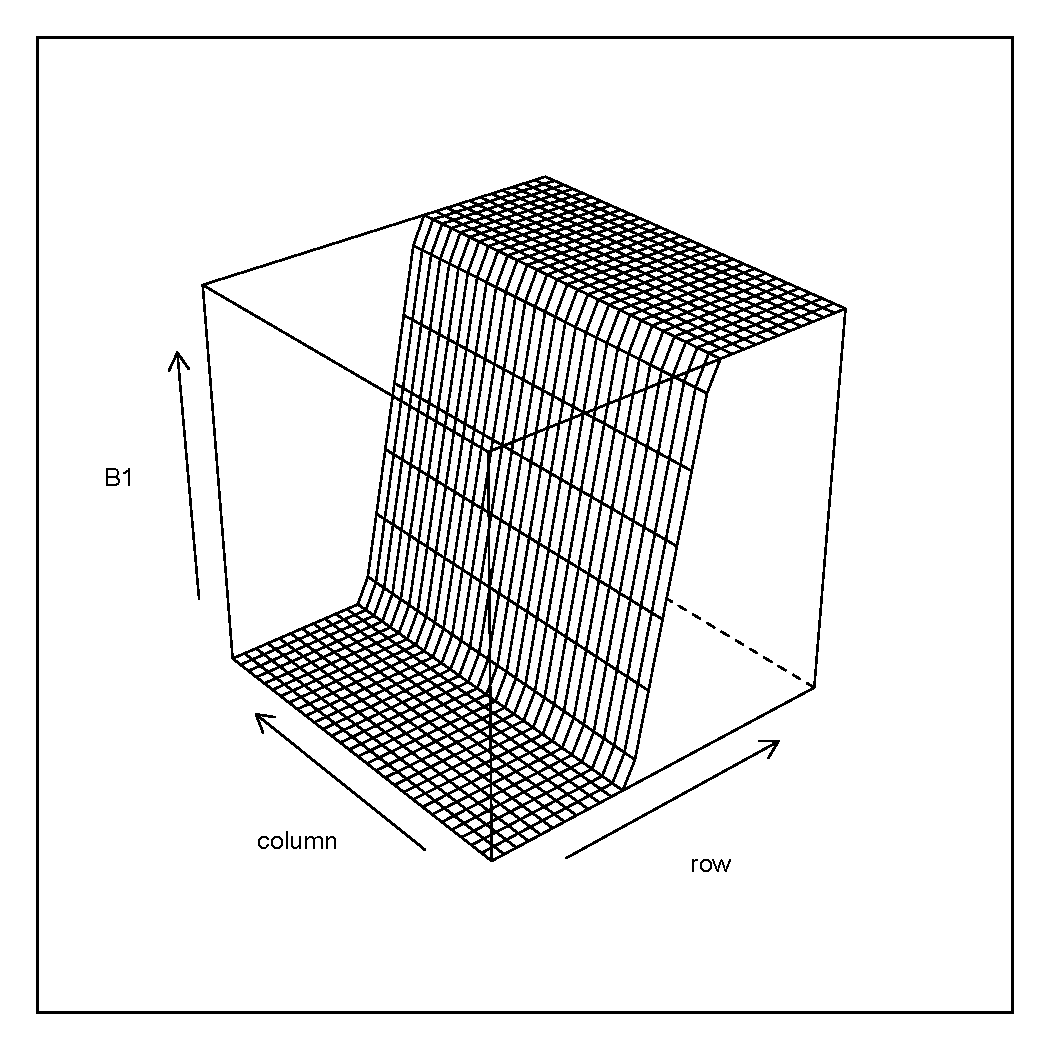
\includegraphics[width=0.33\textwidth]{0_Users_wesley_git_gwr_figures_simulation_step.pdf}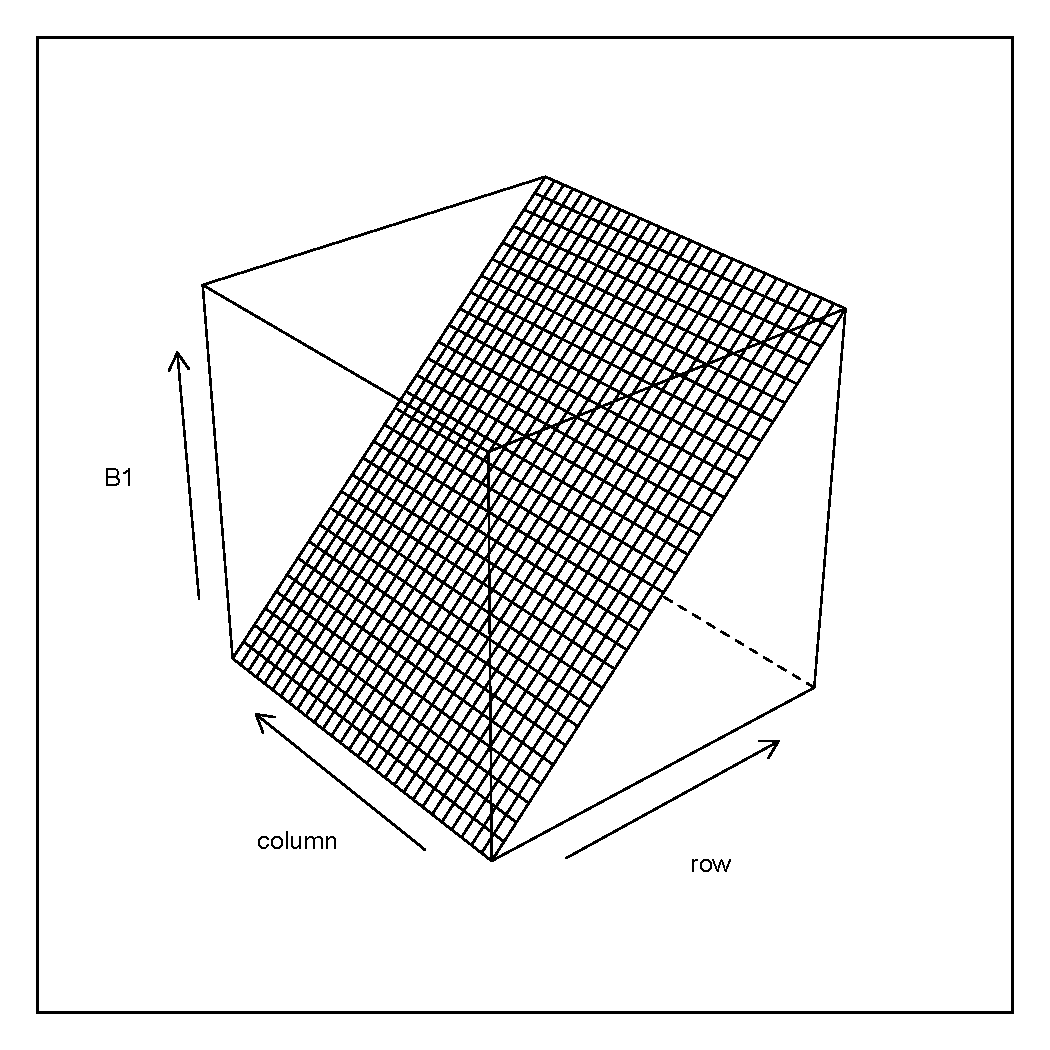
\includegraphics[width=0.33\textwidth]{1_Users_wesley_git_gwr_figures_simulation_gradient.pdf}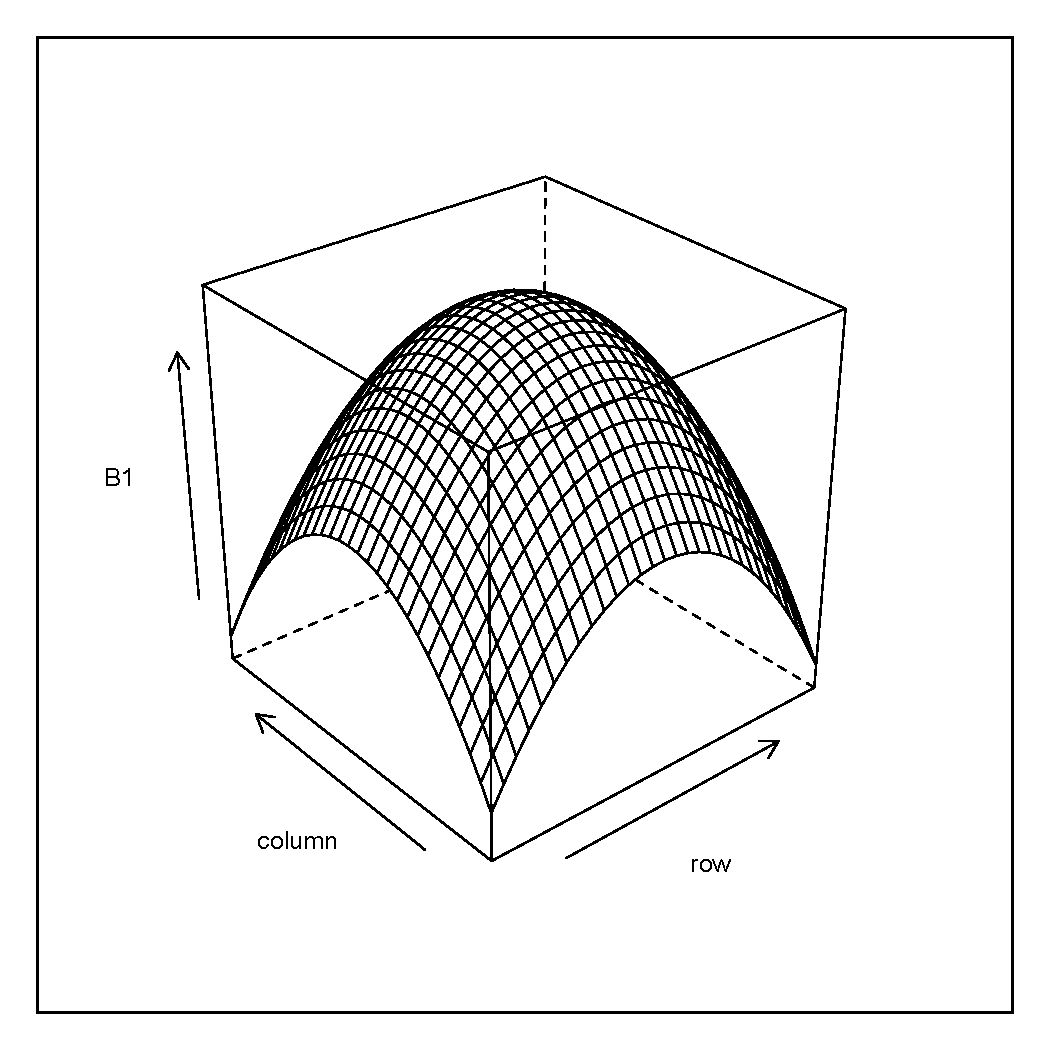
\includegraphics[width=0.33\textwidth]{2_Users_wesley_git_gwr_figures_simulation_parabola.pdf}

\protect\caption{These are, respectively, the step, gradient, and parabola functions
that were used for the coefficient function $\beta_{1}(\bm{s})$ in
the VCR model $y(\bm{s}_{i})=x_{1}(\bm{s}_{i})\beta_{1}(\bm{s}_{i})+\varepsilon(\bm{s}_{i})$
when generating the data for the simulation study.\label{fig:simulation-coefficient-functions}}
\end{figure}


\begin{align}
\nonumber \\
\beta_{gradient}(\bm{s})= & \ \ s_{x}\nonumber \\
\label{eq:simulation-coefficient-functions}
\end{align}


In total, three parameters were varied to produce 18 settings, each
of which was simulated 100 times. There were three functional forms
for the coefficient surface $\beta_{1}(\bm{s})$; data was simulated
both with low ($\rho=0$), medium ($\rho=0.5$), and high ($\rho=0.9$)
correlation between the covariates; and simulations were made with
low ($\sigma_{\varepsilon}^{2}=0.25$) and high ($\sigma_{\varepsilon}^{2}=1$)
variance for the random error term. The simulation settings are enumerated
in Table \ref{tab:simulation-settings}. 

\begin{table}
\begin{tabular}{c|c|c|c}
Setting &
$\beta_{1}(\bm{s})$ &
$\rho$ &
$\sigma_{\varepsilon}^{2}$\tabularnewline
\hline 
1 &
\multirow{6}{*}{step} &
\multirow{2}{*}{0} &
0.25\tabularnewline
\cline{1-1} \cline{4-4} 
2 &
 &  & 1\tabularnewline
\cline{1-1} \cline{3-4} 
3 &
 & \multirow{2}{*}{0.5} &
0.25\tabularnewline
\cline{1-1} \cline{4-4} 
4 &
 &  & 1\tabularnewline
\cline{1-1} \cline{3-4} 
5 &
 & \multirow{2}{*}{0.9} &
0.25\tabularnewline
\cline{1-1} \cline{4-4} 
6 &
 &  & 1\tabularnewline
\hline 
7 &
\multirow{6}{*}{gradient} &
\multirow{2}{*}{0} &
0.25\tabularnewline
\cline{1-1} \cline{4-4} 
8 &
 &  & 1\tabularnewline
\cline{1-1} \cline{3-4} 
9 &
 & \multirow{2}{*}{0.5} &
0.25\tabularnewline
\cline{1-1} \cline{4-4} 
10 &
 &  & 1\tabularnewline
\cline{1-1} \cline{3-4} 
11 &
 & \multirow{2}{*}{0.9} &
0.25\tabularnewline
\cline{1-1} \cline{4-4} 
12 &
 &  & 1\tabularnewline
\hline 
13 &
\multirow{6}{*}{parabola} &
\multirow{2}{*}{0} &
0.25\tabularnewline
\cline{1-1} \cline{4-4} 
14 &
 &  & 1\tabularnewline
\cline{1-1} \cline{3-4} 
15 &
 & \multirow{2}{*}{0.5} &
0.25\tabularnewline
\cline{1-1} \cline{4-4} 
16 &
 &  & 1\tabularnewline
\cline{1-1} \cline{3-4} 
17 &
 & \multirow{2}{*}{0.9} &
0.25\tabularnewline
\cline{1-1} \cline{4-4} 
18 &
 &  & 1\tabularnewline
\end{tabular}

\protect\caption{Listing of the simulation settings used to assess the performance
of LAGR models versus oracle selection and no selection.\label{tab:simulation-settings}}


\end{table}


The results are presented in terms of the mean integrated squared
error (MISE) of the coefficient surface estimates $\hat{\beta}_{1}(\bm{s}),\dots,\hat{\beta}_{5}(\bm{s})$,
the MISE of the fitted response $\hat{y}(\bm{s})$, and the frequency
with which the coefficient surface estimates $\hat{\beta}_{1}(\bm{s}),\dots,\hat{\beta}_{5}(\bm{s})$
in the LAGR model were zero. The performance of LAGR was compared
to that of a VCR model without variable selection, and to a VCR model
with oracular selection. Oracular selection means that exactly the
correct set of covariates was used to fit each local model.


\subsection{Simulation Results}

The MISE of the estimates of $\beta_{1}(\bm{s})$ are in Table \ref{tab:x1-mise}.
Recall that $\beta_{2}(\bm{s}),\dots,\beta_{5}(\bm{s})$ are exactly
zero across the entire domain. Oracle selection will estimate these
coefficients perfectly, so we focus on the comparison between estimation
by LAGR and by the VCR model with no selection. These results show
that for every simulation setting, LAGR estimation is more accurate
than the standard VCR model (Table \ref{tab:x2-x5-mise}).

% latex table generated in R 3.1.0 by xtable 1.7-3 package
% Thu Jul  3 17:26:08 2014
\begin{table}
\centering
\begin{tabular}{rrrr}
  & LAGR & VCR & oracle \\ 
  \hline
1 & \emph{0.02} & 0.02 & \textbf{0.01} \\ 
  2 & \emph{0.03} & 0.03 & \textbf{0.02} \\ 
  3 & \emph{0.02} & 0.02 & \textbf{0.01} \\ 
  4 & \emph{0.03} & 0.05 & \textbf{0.02} \\ 
  5 & \emph{0.03} & 0.05 & \textbf{0.01} \\ 
  6 & \emph{0.12} & 0.17 & \textbf{0.02} \\ 
  7 & 0.01 & \emph{0.01} & \textbf{0.00} \\ 
  8 & 0.03 & \emph{0.02} & \textbf{0.01} \\ 
  9 & 0.01 & \emph{0.01} & \textbf{0.00} \\ 
  10 & 0.04 & \emph{0.03} & \textbf{0.01} \\ 
  11 & \emph{0.03} & 0.04 & \textbf{0.00} \\ 
  12 & \emph{0.14} & 0.14 & \textbf{0.01} \\ 
  13 & 0.01 & \emph{0.01} & \textbf{0.01} \\ 
  14 & 0.03 & \emph{0.02} & \textbf{0.02} \\ 
  15 & 0.01 & \emph{0.01} & \textbf{0.01} \\ 
  16 & 0.03 & \emph{0.03} & \textbf{0.02} \\ 
  17 & \emph{0.02} & 0.04 & \textbf{0.01} \\ 
  18 & 0.17 & \emph{0.14} & \textbf{0.02} \\ 
  \end{tabular}
\caption{The MISE for the estimates of $\beta_1(\bm{s})$ in each simulation setting, under variable selection via LAGR, no variable selection, and oracular variable selection. Highlighting indicates the \textbf{lowest} and \emph{next-lowest} MISE.} 
\label{tab:x1-mise}
\end{table}


% latex table generated in R 3.1.0 by xtable 1.7-3 package
% Thu Jul  3 17:26:15 2014
\begin{table}
\centering
\begin{tabular}{rrr}
  & LAGR & VCR \\ 
  \hline
1 & \textbf{0.000} & 0.005 \\ 
  2 & \textbf{0.001} & 0.019 \\ 
  3 & \textbf{0.000} & 0.008 \\ 
  4 & \textbf{0.002} & 0.030 \\ 
  5 & \textbf{0.003} & 0.041 \\ 
  6 & \textbf{0.017} & 0.150 \\ 
  7 & \textbf{0.000} & 0.005 \\ 
  8 & \textbf{0.001} & 0.018 \\ 
  9 & \textbf{0.000} & 0.008 \\ 
  10 & \textbf{0.002} & 0.032 \\ 
  11 & \textbf{0.004} & 0.037 \\ 
  12 & \textbf{0.018} & 0.147 \\ 
  13 & \textbf{0.000} & 0.005 \\ 
  14 & \textbf{0.001} & 0.018 \\ 
  15 & \textbf{0.000} & 0.008 \\ 
  16 & \textbf{0.002} & 0.031 \\ 
  17 & \textbf{0.004} & 0.038 \\ 
  18 & \textbf{0.027} & 0.146 \\ 
  \end{tabular}
\caption{The MISE for the estimates of $\beta_2(\bm{s}),\dots,\beta_5(\bm{s})$ in each simulation setting, under variable selection via LAGR and no variable selection. Highlighting indicates the \textbf{lowest} MISE.} 
\label{tab:x2-x5-mise}
\end{table}


% latex table generated in R 3.1.0 by xtable 1.7-3 package
% Thu Jul  3 17:26:17 2014
\begin{table}
\centering
\begin{tabular}{rr}
  & Frequency of exact zero \\ 
  \hline
1 & 0.97 \\ 
  2 & 0.96 \\ 
  3 & 0.96 \\ 
  4 & 0.92 \\ 
  5 & 0.86 \\ 
  6 & 0.85 \\ 
  7 & 0.96 \\ 
  8 & 0.95 \\ 
  9 & 0.94 \\ 
  10 & 0.92 \\ 
  11 & 0.80 \\ 
  12 & 0.85 \\ 
  13 & 0.97 \\ 
  14 & 0.94 \\ 
  15 & 0.95 \\ 
  16 & 0.88 \\ 
  17 & 0.79 \\ 
  18 & 0.78 \\ 
  \end{tabular}
\caption{Proportion of local models under each setting in which the coefficients $\beta_2(\bm{s}),\dots,\beta_5(\bm{s})$ are estimated as exactly zero.} 
\label{tab:pzero}
\end{table}


% latex table generated in R 3.1.0 by xtable 1.7-3 package
% Thu Jul  3 17:26:19 2014
\begin{table}
\centering
\begin{tabular}{rrrr}
  & LAGR & VCR & oracle \\ 
  \hline
1 & \emph{0.25} & 0.26 & \textbf{0.25} \\ 
  2 & \emph{1.00} & \textbf{1.00} & 0.99 \\ 
  3 & \emph{0.26} & 0.26 & \textbf{0.25} \\ 
  4 & \emph{0.99} & \textbf{1.00} & 0.98 \\ 
  5 & \emph{0.27} & 0.30 & \textbf{0.25} \\ 
  6 & \emph{1.08} & 1.14 & \textbf{0.98} \\ 
  7 & \emph{0.25} & \textbf{0.25} & 0.25 \\ 
  8 & \textbf{0.99} & \emph{0.99} & 0.97 \\ 
  9 & \emph{0.25} & \textbf{0.25} & 0.24 \\ 
  10 & \emph{1.00} & \textbf{1.00} & 0.97 \\ 
  11 & \emph{0.27} & 0.28 & \textbf{0.24} \\ 
  12 & \emph{1.09} & 1.12 & \textbf{0.97} \\ 
  13 & \emph{0.25} & \textbf{0.25} & 0.25 \\ 
  14 & \textbf{1.00} & \emph{1.00} & 0.98 \\ 
  15 & \textbf{0.25} & 0.25 & \emph{0.25} \\ 
  16 & \textbf{1.00} & \emph{1.00} & 0.97 \\ 
  17 & \emph{0.26} & 0.28 & \textbf{0.24} \\ 
  18 & 1.13 & \emph{1.12} & \textbf{0.98} \\ 
  \end{tabular}
\caption{The MISE for the fitted output in each simulation setting, under variable selection via LAGR, no variable selection, and oracular variable selection. Highlighting indicates the \textbf{closest} and \emph{next-closest} to the actual error variance $\sigma_\varepsilon^2$ for that setting.} 
\label{tab:misey}
\end{table}


From Table \ref{tab:pzero} we see that LAGR has good ability to identify
zero-coefficient covariates. The frequency with which $\beta_{2}(\bm{s}),\dots,\beta_{5}(\bm{s})$
were dropped from the LAGR models ranged from 0.78
to 0.97. The MISE of the fitted $\hat{y}(\bm{s})$
is listed in Table \ref{tab:misey}, where the highlighting is based
on which methods estimate an error variance that is closest to the
known truth for the simulation. The results are all very similar to
each other, indicating that no method was consistently better than
the others in this simulation at fitting the model output

The proposed LAGR method was accurate in selection and estimation,
with estimation accuracy for $\beta_{1}(\bm{s})$ about equal to that
of the VCR model with no selection, and with consistently better accuracy
for estimating $\beta_{2}(\bm{s}),\dots,\beta_{5}(\bm{s})$.

There was minimal difference in the performance of the proposed LAGR
method between low ($\sigma_{\varepsilon}=0.5$) and high ($\sigma_{\varepsilon}=1$)
error variance, and between no ($\rho=0$) and moderate ($\rho=0.5$)
correlation among the predictor variables. But the selection and estimation
accuracy did decline when there was high ($\rho=0.9$) correlation
among the predictor variables.


\section{Data Example\label{sec:example}}

The proposed LAGR estimation method was used to estimate the coefficients
in a VCR model of the effect of some covariates on the price of homes
in Boston. The data source is the Boston house price data set, which
is based on the 1970 U.S. census \citet{Harrison-Rubinfeld-1978,Gilley-Pace-1996,Pace-Gilley-1997}.
In the data, we have the median price of homes sold in 506 census
tracts (MEDV), along with the following potential covariates: CRIM
(the per-capita crime rate in the tract), RM (the mean number of rooms
for houses sold in the tract), RAD (an index of how accessible the
tract is from Boston's radial roads), TAX (the property tax per \$10,000
of property value), and LSTAT (the percentage of the tract's residents
who are considered ``lower status''). The bandwidth parameter was
set to 0.2 for a nearest neighbors-type bandwidth, meaning that the
sum of kernel weights for each local model was 20\% of the total number
of observations. The kernel used was the Epanechnikov kernel.


\subsection{Results}

\begin{figure}

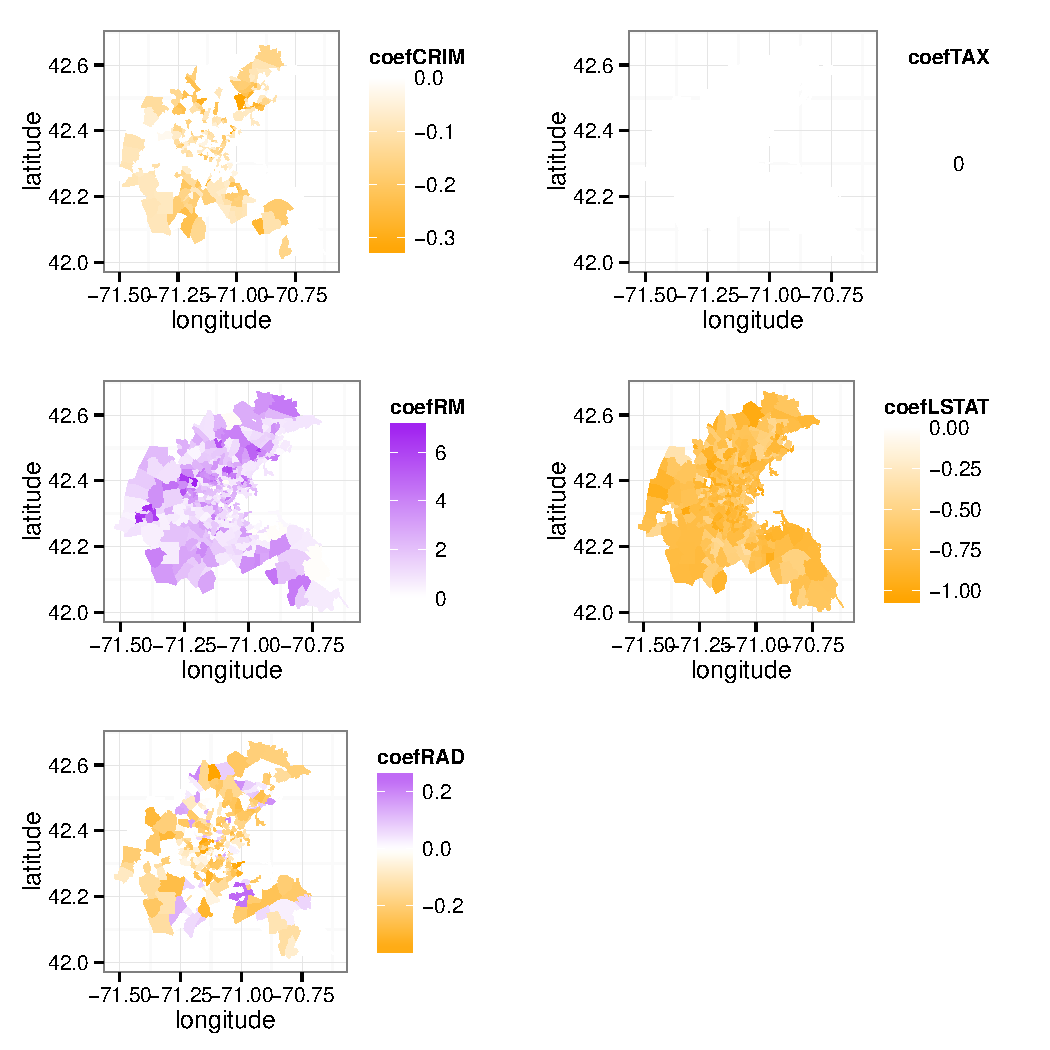
\includegraphics[width=\maxwidth]{figure/boston-plots} 


\caption{The LAGR estimates of coefficients for the Boston house price data.\label{fig:boston-lagr-coefs}}
\end{figure}

Estimates of the regression coefficients are plotted in Figure \ref{fig:boston-lagr-coefs}.
One interesting result is that LAGR indicates that the TAX variable
was nowhere an important predictor of the median house price. Another
is that the coefficients of CRIM and LSTAT are everywhere negative
or zero (meaning that the increasing the crime rate or proportion
of lower-status individuals reduces the median house price where the
effect is discernable) and that of RM is positive (meaning that when
the average house in a tract has more rooms, the median house will
be more expensive). The coefficient of RAD is positive in some areas
and negative in others. This indicates that there are parts of Boston
where access to radial roads is positively associated with an increase
in the median house price and parts where the association is negative.

There is not an obvious spatial pattern to the local coefficients
for RAD - there are more tracts with negative coefficients than positive,
and the positive coefficients do appear to be clustered, but the tracts
with positive coefficients are also adjacent to tracts with negative
coefficients. Indeed, there is not an obvious spatial pattern to any
of the coefficient surfaces except for TAX, which is zero everywhere.

% latex table generated in R 3.1.0 by xtable 1.7-3 package
% Thu Jul  3 17:26:26 2014
\begin{table}
\centering
\begin{tabular}{rrrr}
  & Mean & SD & Prop. zero \\ 
  \hline
CRIM & -0.07 & 0.08 & 0.49 \\ 
  RM & 1.92 & 1.43 & 0.02 \\ 
  RAD & -0.08 & 0.13 & 0.37 \\ 
  TAX & 0.00 & 0.00 & 1.00 \\ 
  LSTAT & -0.72 & 0.16 & 0.01 \\ 
  \end{tabular}
\caption{The mean, standard deviation, and proportion of zeros among the local coefficients in a model for the median house price in census tracts in Boston, with coefficients selected and fitted by LAGR.} 
\label{tab:boston-coefs-lagr}
\end{table}


A summary of the local coefficients is in Table \ref{tab:boston-coefs-lagr}.
It indicates that RM is the only predictor variable with a positive
mean of the local coefficients, but also that the mean of the local
coefficients of RM is the largest coefficient - at 1.92,
it is more than twice as large in magnitude as the mean local coefficient
of LSTAT (\ensuremath{-0.72}),
which is second-largest.

The coefficient of the CRIM variable was estimated to be exactly zero
at 49\%
of the locations. The percentage for the RAD variable was 37\%.

In their example using the same data, \citet{Sun-Yan-Zhang-Lu-2014}
estimated that the coefficients of RAD annd LSTAT should be constant,
at 0.36 and -0.45, respectively. That conclusion differs from our
result, which says that the mean local coefficient of RAD is actually
negative (\ensuremath{-0.08}), while
our mean fitted local coefficient for LSTAT was more negative than
the estimate of \citet{Sun-Yan-Zhang-Lu-2014}.

\appendix

\section{Proofs of Theorems\label{app:proofs} }
\begin{proof}[Proof of Theorem \ref{theorem:normality}]

\end{proof}
Let $V_{4}^{(n)}(\bm{u})=\mathcal{J}\left(\bm{\zeta}(\bm{s})+h^{-1}n^{-1/2}\bm{u}\right)-\mathcal{J}\left(\bm{\zeta}(\bm{s})\right)$.
Then we have that 
\begin{align}
\mkern-36muV_{4}^{(n)}(\bm{u})= & (1/2)\left[\bm{Y}-\bm{Z}(\bm{s})\left\{ \bm{\zeta}(\bm{s})+h^{-1}n^{-1/2}\bm{u}\right\} \right]^{T}\bm{W}(\bm{s})\left[\bm{Y}-\bm{Z}(\bm{s})\left\{ \bm{\zeta}(\bm{s})+h^{-1}n^{-1/2}\bm{u}\right\} \right]\notag\\
 & +\sum_{j=1}^{p}\phi_{j}(\bm{s})\|\bm{\zeta}_{j}(\bm{s})+h^{-1}n^{-1/2}\bm{u}_{j}\|\notag\\
 & -(1/2)\left\{ \bm{Y}-\bm{Z}(\bm{s})\bm{\zeta}(\bm{s})\right\} ^{T}\bm{W}(\bm{s})\left\{ \bm{Y}-\bm{Z}(\bm{s})\bm{\zeta}(\bm{s})\right\} -\sum_{j=1}^{p}\phi_{j}(\bm{s})\|\bm{\zeta}_{j}(\bm{s})\|\notag\\
 & \mkern-36mu=(1/2)\bm{u}^{T}\left\{ h^{-2}n^{-1}\bm{Z}^{T}(\bm{s})\bm{W}(\bm{s})\bm{Z}(\bm{s})\right\} \bm{u}\notag\\
 & -\bm{u}^{T}\left[h^{-1}n^{-1/2}\bm{Z}^{T}(\bm{s})\bm{W}(\bm{s})\left\{ \bm{Y}-\bm{Z}(\bm{s})\bm{\zeta}(\bm{s})\right\} \right]\\
 & +\sum_{j=1}^{p}n^{-1/2}\phi_{j}(\bm{s})n^{1/2}\left\{ \|\bm{\zeta}_{j}(\bm{s})+h^{-1}n^{-1/2}\bm{u}_{j}\|-\|\bm{\zeta}_{j}(\bm{s})\|\right\} 
\end{align}


The limiting behavior of the third term differs between the cases
$j\le p_{0}$ and $j>p_{0}$.


\paragraph{Case $j\le p_{0}$:}

If $j\le p_{0}$, then $n^{-1/2}\phi_{j}(\bm{s})\to n^{-1/2}\lambda_{n}(\bm{s})\|\bm{\zeta}_{j}(\bm{s})\|^{-\gamma}$
and $|\sqrt{n}\left\{ \|\bm{\zeta}_{j}(\bm{s})+h^{-1}n^{-1/2}\bm{u}_{j}\|-\|\bm{\zeta}_{j}(\bm{s})\|\right\} |\le h^{-1}\|\bm{u}_{j}\|$.
Thus, 
\[
\lim\limits _{n\to\infty}\phi_{j}(\bm{s})\left\{ \|\bm{\zeta}_{j}(\bm{s})+h^{-1}n^{-1/2}\bm{u}_{j}\|-\|\bm{\zeta}_{j}(\bm{s})\|\right\} \le h^{-1}n^{-1/2}\phi_{j}(\bm{s})\|\bm{u}_{j}\|\le h^{-1}n^{-1/2}a_{n}\|\bm{u}_{j}\|\to0
\]



\paragraph{Case $j>p_{0}$:}

If $j>p_{0}$, then $\phi_{j}(\bm{s})\left\{ \|\bm{\zeta}_{j}(\bm{s})+h^{-1}n^{-1/2}\bm{u}_{j}\|-\|\bm{\zeta}_{j}(\bm{s})\|\right\} =\phi_{j}(\bm{s})h^{-1}n^{-1/2}\|\bm{u}_{j}\|$.

Since $h=O(n^{-1/6})$, if $hn^{-1/2}b_{n}\xrightarrow{p}\infty$,
then $h^{-1}n^{-1/2}b_{n}\xrightarrow{p}\infty$.

Now, if $\|\bm{u}_{j}\|\ne0$, then 
\[
h^{-1}n^{-1/2}\phi_{j}(\bm{s})\|\bm{u}_{j}\|\ge h^{-1}n^{-1/2}b_{n}\|\bm{u}_{j}\|\to\infty.
\]
On the other hand, if $\|\bm{u}_{j}\|=0$, then $h^{-1}n^{-1/2}\phi_{j}(\bm{s})\|\bm{u}_{j}\|=0$.

Thus, the limit of $V_{4}^{(n)}(\bm{u})$ is the same as the limit
of $V_{4}^{*(n)}(\bm{u})$ where

\[
V_{4}^{*(n)}(\bm{u})=(1/2)\bm{u}^{T}\left\{ h^{-2}n^{-1}\bm{Z}^{T}(\bm{s})\bm{W}(\bm{s})\bm{Z}(\bm{s})\right\} \bm{u}-\bm{u}^{T}\left[h^{-1}n^{-1/2}\bm{Z}^{T}(\bm{s})\bm{W}(\bm{s})\left\{ \bm{Y}-\bm{Z}(\bm{s})\bm{\zeta}(\bm{s})\right\} \right].
\]


if $\|\bm{u}_{j}\|=0\;\forall j>p_{0}$ and $V_{4}^{*(n)}(\bm{u})=\infty$
otherwise. It follows that $V_{4}^{*(n)}(\bm{u})$ is convex and its
unique minimizer $\hat{\bm{u}}^{(n)}$ is found by solving the equation:

\begin{align}
\bm{0}_{3p} & =\left\{ h^{-2}n^{-1}\bm{Z}(\bm{s})^{T}\bm{W}(\bm{s})\bm{Z}(\bm{s})\right\} \hat{\bm{u}}^{(n)}-\left[h^{-1}n^{-1/2}\bm{Z}(\bm{s})^{T}\bm{W}(\bm{s})\left\{ \bm{Y}-\bm{Z}(\bm{s})\bm{\zeta}(\bm{s})\right\} \right].\label{eq:limit}
\end{align}


That is, 

\[
\hat{\bm{u}}^{(n)}=\left\{ n^{-1}\bm{Z}(\bm{s})^{T}\bm{W}(\bm{s})\bm{Z}(\bm{s})\right\} ^{-1}\left[hn^{-1/2}\bm{Z}(\bm{s})^{T}\bm{W}(\bm{s})\left\{ \bm{Y}-\bm{Z}(\bm{s})\bm{\zeta}(\bm{s})\right\} \right].
\]


By the epiconvergence results of \citet{Geyer-1994} and \citet{Knight-Fu-2000},
the minimizer of the limiting function is the limit of the minimizers
$\hat{\bm{u}}^{(n)}$. Since, by Lemma 2 of \citet{Sun-Yan-Zhang-Lu-2014},

\begin{equation}
\hat{\bm{u}}^{(n)}\xrightarrow{d}N\left(\frac{\kappa_{2}h^{2}}{2\kappa_{0}}\{\nabla_{uu}^{2}\bm{\zeta}_{j}(\bm{s})+\nabla_{vv}^{2}\bm{\zeta}_{j}(\bm{s})\},f(\bm{s})\kappa_{0}^{-2}\nu_{0}\sigma^{2}\Psi^{-1}\right)
\end{equation}
the result of Theorem \ref{theorem:normality-glm} follows.
\begin{proof}[Proof of Theorem \ref{theorem:selection}]


We showed in Theorem \ref{theorem:normality} that $\hat{\bm{\zeta}}_{j}(\bm{s})\xrightarrow{p}\bm{\zeta}_{j}(\bm{s})+\frac{\kappa_{2}h^{2}}{2\kappa_{0}}\{\nabla_{uu}^{2}\bm{\zeta}_{j}(\bm{s})+\nabla_{vv}^{2}\bm{\zeta}_{j}(\bm{s})\}$,
so to complete the proof of selection consistency, it only remains
to show that $P\left\{ \hat{\bm{\zeta}}_{j}(\bm{s})=\undertilde{0}\right\} \to1$
if $j>p_{0}$.
\end{proof}
The proof is by contradiction. Without loss of generality, we consider
only the case $j=p$.

Assume $\|\hat{\bm{\zeta}}_{p}(\bm{s})\|\ne\undertilde{0}$. Then
$Q\left\{ \bm{\zeta}(\bm{s})\right\} $ is differentiable w.r.t. $\bm{\zeta}_{p}(\bm{s})$
and is minimized where 
\begin{align}
\undertilde{0} & =\bm{Z}_{p}^{T}(\bm{s})\bm{W}(\bm{s})\left\{ \bm{Y}-\bm{Z}_{-p}(\bm{s})\hat{\bm{\zeta}}_{-p}(\bm{s})-\bm{Z}_{p}(\bm{s})\hat{\bm{\zeta}}_{p}(\bm{s})\right\} -\phi_{p}(\bm{s})\frac{\hat{\bm{\zeta}}_{p}(\bm{s})}{\|\hat{\bm{\zeta}}_{p}(\bm{s})\|}\notag\\
 & =\bm{Z}_{p}^{T}(\bm{s})\bm{W}(\bm{s})\left[\bm{Y}-\bm{Z}(\bm{s})\bm{\zeta}(\bm{s})-\frac{h^{2}\kappa_{2}}{2\kappa_{0}}\left\{ \nabla_{uu}^{2}\bm{\zeta}(\bm{s})+\nabla_{vv}^{2}\bm{\zeta}(\bm{s})\right\} \right]\notag\\
 & \mkern+72mu+\bm{Z}_{p}^{T}(\bm{s})\bm{W}(\bm{s})\bm{Z}_{-p}(\bm{s})\left[\bm{\zeta}_{-p}(\bm{s})+\frac{h^{2}\kappa_{2}}{2\kappa_{0}}\left\{ \nabla_{uu}^{2}\bm{\zeta}_{-p}(\bm{s})+\nabla_{vv}^{2}\bm{\zeta}_{-p}(\bm{s})\right\} -\hat{\bm{\zeta}}_{-p}(\bm{s})\right]\notag\\
 & \mkern+72mu+\bm{Z}_{p}^{T}(\bm{s})\bm{W}(\bm{s})\bm{Z}_{p}(\bm{s})\left[\bm{\zeta}_{p}(\bm{s})+\frac{h^{2}\kappa_{2}}{2\kappa_{0}}\left\{ \nabla_{uu}^{2}\bm{\zeta}_{p}(\bm{s})+\nabla_{vv}^{2}\bm{\zeta}_{p}(\bm{s})\right\} -\hat{\bm{\zeta}}_{p}(\bm{s})\right]\notag\\
 & \mkern+72mu-\phi_{p}(\bm{s})\frac{\hat{\bm{\zeta}}_{p}(\bm{s})}{\|\hat{\bm{\zeta}}_{p}(\bm{s})\|}\notag\\
\end{align}


Thus, 
\begin{align}
\frac{h}{\sqrt{n}}\phi_{p}(\bm{s})\frac{\hat{\bm{\zeta}}_{p}(\bm{s})}{\|\hat{\bm{\zeta}}_{p}(\bm{s})\|}=\label{eq:selection}\\
 & \bm{Z}_{p}^{T}(\bm{s})\bm{W}(\bm{s})\frac{h}{\sqrt{n}}\left[\bm{Y}-\bm{Z}(\bm{s})\bm{\zeta}(\bm{s})-\frac{h^{2}\kappa_{2}}{2\kappa_{0}}\left\{ \nabla_{uu}^{2}\bm{\zeta}(\bm{s})+\nabla_{vv}^{2}\bm{\zeta}(\bm{s})\right\} \right]\\
 & +\left\{ n^{-1}\bm{Z}_{p}^{T}(\bm{s})\bm{W}(\bm{s})\bm{Z}_{-p}(\bm{s})\right\} h\sqrt{n}\left[\bm{\zeta}_{-p}(\bm{s})+\frac{h^{2}\kappa_{2}}{2\kappa_{0}}\left\{ \nabla_{uu}^{2}\bm{\zeta}_{-p}(\bm{s})+\nabla_{vv}^{2}\bm{\zeta}_{-p}(\bm{s})\right\} -\hat{\bm{\zeta}}_{-p}(\bm{s})\right]\\
 & +\left\{ n^{-1}\bm{Z}_{p}^{T}(\bm{s})\bm{W}(\bm{s})\bm{Z}_{p}(\bm{s})\right\} h\sqrt{n}\left[\bm{\zeta}_{p}(\bm{s})+\frac{h^{2}\kappa_{2}}{2\kappa_{0}}\left\{ \nabla_{uu}^{2}\bm{\zeta}_{p}(\bm{s})+\nabla_{vv}^{2}\bm{\zeta}_{p}(\bm{s})\right\} -\hat{\bm{\zeta}}_{p}(\bm{s})\right]
\end{align}


From Lemma 2 of \citet{Sun-Yan-Zhang-Lu-2014}, $n^{-1}\bm{Z}_{p}^{T}(\bm{s})\bm{W}(\bm{s})\bm{Z}_{-p}(\bm{s})=O_{p}(1)$
and $n^{-1}\bm{Z}_{p}^{T}(\bm{s})\bm{W}(\bm{s})\bm{Z}_{p}(\bm{s})=O_{p}(1)$.

From Theorem 3 of \citet{Sun-Yan-Zhang-Lu-2014}, we have that $h\sqrt{n}\left[\hat{\bm{\zeta}}_{-p}(\bm{s})-\bm{\zeta}_{-p}(\bm{s})-\frac{h^{2}\kappa_{2}}{2\kappa_{0}}\left\{ \nabla_{uu}^{2}\zeta_{-p}(\bm{s})+\nabla_{vv}^{2}\zeta_{-p}(\bm{s})\right\} \right]=O_{p}(1)$
and $h\sqrt{n}\left[\hat{\bm{\zeta}}_{p}(\bm{s})-\bm{\zeta}_{p}(\bm{s})-\frac{h^{2}\kappa_{2}}{2\kappa_{0}}\left\{ \nabla_{uu}^{2}\zeta_{p}(\bm{s})+\nabla_{vv}^{2}\zeta_{p}(\bm{s})\right\} \right]=O_{p}(1)$.

Thus, the second and third terms of the sum in (\ref{eq:selection})
are $O_{p}(1)$, and we showed in the proof of Theorem \ref{theorem:normality}
that 

\[
h\sqrt{n}\bm{Z}_{p}^{T}(\bm{s})\bm{W}(\bm{s})\left[\bm{Y}-\bm{Z}(\bm{s})\bm{\zeta}(\bm{s})-\frac{h^{2}\kappa_{2}}{2\kappa_{0}}\left\{ \nabla_{uu}^{2}\bm{\zeta}(\bm{s})+\nabla_{vv}^{2}\bm{\zeta}(\bm{s})\right\} \right]=O_{p}(1).
\]


The three terms of the sum to the right of the equals sign in (\ref{eq:selection})
are $O_{p}(1)$, so for $\hat{\bm{\zeta}}_{p}(\bm{s})$ to be a solution,
we must have that $hn^{-1/2}\phi_{p}(\bm{s})\hat{\bm{\zeta}}_{p}(\bm{s})/\|\hat{\bm{\zeta}}_{p}(\bm{s})\|=O_{p}(1)$.

But since by assumption $\hat{\bm{\zeta}}_{p}(\bm{s})\ne\undertilde{0}$,
there must be some $k\in\{1,2,3\}$ such that $|\hat{\zeta}_{p_{k}}(\bm{s})|=\max\{|\hat{\zeta}_{p_{k'}}(\bm{s})|:1\le k'\le3\}$.
And for this $k$, we have that $|\hat{\zeta}_{p_{k}}(\bm{s})|/\|\hat{\bm{\zeta}}_{p}(\bm{s})\|\ge1/\sqrt{3}>0$.

Now since $hn^{-1/2}b_{n}\to\infty$, we have that $hn^{-1/2}\phi_{p}(\bm{s})\hat{\bm{\zeta}}_{p}(\bm{s})/\|\hat{\bm{\zeta}}_{p}(\bm{s})\|\ge hb_{n}/\sqrt{3n}\to\infty$
and therefore the term to the left of the equals sign dominates the
sum to the right of the equals sign in (\ref{eq:selection}). Thus,
for large enough $n$, $\hat{\bm{\zeta}}_{p}(\bm{s})\ne\undertilde{0}$
cannot maximize $\mathcal{J}$.

Thus, $P\left\{ \hat{\bm{\zeta}}_{(b)}(\bm{s})=\undertilde{0}\right\} \to1$. 

\begin{comment}
\begin{proof}[Proof of theorem \ref{theorem:normality-glm}]


Define the $q$-functions to be the derivatives of the quasi-likelihood:
$q_{j}(t,y)=\left(\partial/\partial t\right)^{j}Q\left(g^{-1}\left(t\right),y\right)$.
Then $q_{1}\left(\eta\left(\bm{s}\right),\mu\left(\bm{s}\right)\right)=0$
and $q_{2}\left(\eta\left(\bm{s}\right),\mu\left(\bm{s}\right)\right)=-b''\left(\eta\left(\bm{s}\right)\right)$.
Also define $\bar{\eta}_{i}\left(\right)$
\end{proof}
Define $H^{(n)}(\bm{u})$ to be 
\begin{align}
H^{(n)}(\bm{u})= & \mathcal{J}^{*}\left(\bm{\zeta}(\bm{s})+h^{-1}n^{-1/2}\bm{u}\right)-\mathcal{J}^{*}\left(\bm{\zeta}(\bm{s})\right)\label{eq:consistency-glm}
\end{align}


Let $\bar{\eta}_{i}\left(\bm{s}\right)=\left\{ \bm{Z}(\bm{s}_{i})\right\} _{i}^{T}\bm{\zeta}(\bm{s})$
be the fitted value of $\eta\left(\bm{s}_{i}\right)$ based on the
coefficients at $\bm{s}_{i}$. Then the Taylor expansion of $\mathcal{J}^{*}\left\{ \bm{\zeta}(\bm{s})+h^{-1}n^{-1/2}\bm{u}\right\} $
around $\bm{\zeta}\left(\bm{s}\right)$ is:

\begin{align*}
\mathcal{J}^{*}\left(\bm{\zeta}(\bm{s})+h^{-1}n^{-1/2}\bm{u}\right)= & \mathcal{J}^{*}\left(\bm{\zeta}(\bm{s})\right)\\
 & +h^{-1}n^{-1/2}\sum_{i=1}^{n}K_{h}(\|\bm{s}-\bm{s}_{i}\|)q_{1}\left(\bar{\eta}_{i}\left(\bm{s}\right),y\left(\bm{s}_{i}\right)\right)\left\{ \bm{Z}(\bm{s}_{i})\right\} _{i}^{T}\bm{u}\\
 & +h^{-2}n^{-1}\sum_{i=1}^{n}K_{h}(\|\bm{s}-\bm{s}_{i}\|)q_{2}\left(\bar{\eta}_{i}\left(\bm{s}\right),y\left(\bm{s}_{i}\right)\right)\bm{u}^{T}\left\{ \bm{Z}(\bm{s}_{i})\right\} _{i}\left\{ \bm{Z}(\bm{s}_{i})\right\} _{i}^{T}\bm{u}\\
 & +h^{-3}n^{-3/2}\sum_{i=1}^{n}K_{h}(\|\bm{s}-\bm{s}_{i}\|)q_{3}\left(\tilde{\eta}_{i},y\left(\bm{s}_{i}\right)\right)\left[\left\{ \bm{Z}(\bm{s}_{i})\right\} _{i}^{T}\bm{u}\right]^{3}\\
 & +\sum_{j=1}^{p}\phi_{j}(\bm{s})\|\bm{\zeta}_{j}(\bm{s})+h^{-1}n^{-1/2}\bm{u}\|
\end{align*}


where $\tilde{\eta}_{i}$ is between $\bar{\eta}_{i}\left(\bm{s}\right)$
and $\bar{\eta}_{i}\left(\bm{s}\right)+h^{-1}n^{-1/2}\left\{ \bm{Z}(\bm{s}_{i})\right\} _{i}^{T}\bm{u}$.
Let $A_{1}\left(\bm{s}\right)=\sum_{i=1}^{n}K_{h}(\|\bm{s}-\bm{s}_{i}\|)q_{1}\left(\left\{ \bm{Z}(\bm{s}_{i})\right\} _{i}^{T}\bm{\zeta}(\bm{s}),y\left(\bm{s}_{i}\right)\right)\left\{ \bm{Z}(\bm{s}_{i})\right\} _{i}^{T}$
and $A_{2}\left(\bm{s}\right)=\sum_{i=1}^{n}K_{h}(\|\bm{s}-\bm{s}_{i}\|)q_{2}\left(\left\{ \bm{Z}(\bm{s}_{i})\right\} _{i}^{T}\bm{\zeta}(\bm{s}),y\left(\bm{s}_{i}\right)\right)\left\{ \bm{Z}(\bm{s}_{i})\right\} _{i}\left\{ \bm{Z}(\bm{s}_{i})\right\} _{i}^{T}$.
Now,

\begin{align}
H^{(n)}(\bm{u})= & h^{-1}n^{-1/2}A_{1}\left(\bm{s}\right)\bm{u}\label{eq:glm-Taylor-expansion}\\
 & +h^{-2}n^{-1}\bm{u}^{T}A_{2}\left(\bm{s}\right)\bm{u}\\
 & +h^{-3}n^{-3/2}\sum_{i=1}^{n}K_{h}(\|\bm{s}-\bm{s}_{i}\|)q_{3}\left(\tilde{\eta}_{i},y\left(\bm{s}_{i}\right)\right)\left[\left\{ \bm{Z}(\bm{s}_{i})\right\} _{i}^{T}\bm{u}\right]^{3}\\
 & +\sum_{j=1}^{p}\phi_{j}(\bm{s})\left\{ \|\bm{\zeta}_{j}(\bm{s})+h^{-1}n^{-1/2}\bm{u}\|-\|\bm{\zeta}_{j}(\bm{s})\|\right\} \nonumber 
\end{align}


where $\tilde{\bm{\zeta}_{i}}$ lies between $\bm{\zeta}(\bm{s})$
and $\bm{\zeta}(\bm{s})+h^{-1}n^{-1/2}\bm{u}$. Now the difference
$H^{(n)}(\bm{u})=\mathcal{J}^{*}\left(\bm{\zeta}(\bm{s})+h^{-1}n^{-1/2}\bm{u}\right)-\mathcal{J}^{*}\left(\bm{\zeta}(\bm{s})\right)$
is 

\begin{align*}
H^{(n)}(\bm{u})= & h^{-1}n^{-1/2}\bm{u}\sum_{i=1}^{n}q_{1}\left(\bm{Z}'(\bm{s}_{i})\bm{\zeta}(\bm{s}),Y\left(\bm{s}_{i}\right)\right)K_{h}\left(\|\bm{s}-\bm{s}_{i}\|\right)\\
 & +h^{-2}n^{-1}\bm{u}'\bm{u}\sum_{i=1}^{n}q_{2}\left(\bm{Z}'(\bm{s}_{i})\bm{\zeta}(\bm{s}),Y\left(\bm{s}_{i}\right)\right)K_{h}\left(\|\bm{s}-\bm{s}_{i}\|\right)\\
 & +\left(h^{-1}n^{-1/2}\bm{u}\right)^{3}\sum_{i=1}^{n}q_{3}\left(\tilde{\eta}_{i},Y\left(\bm{s}_{i}\right)\right)K_{h}\left(\|\bm{s}-\bm{s}_{i}\|\right)\\
 & +\sum_{j=1}^{p}\phi_{j}(\bm{s})\left\{ \|\bm{\zeta}_{j}(\bm{s})+h^{-1}n^{-1/2}\bm{u}\|-\|\bm{\zeta}_{j}(\bm{s})\|\right\} 
\end{align*}


The limiting behavior of the fourth differs term between the cases
$j\le p_{0}$ and $j>p_{0}$:


\paragraph{Case $j\le p_{0}$}

If $j\le p_{0}$ then $n^{-1/2}\phi_{j}(\bm{s})\to n^{-1/2}\lambda_{n}(\bm{s})\|\bm{\zeta}_{j}(\bm{s})\|^{-\gamma}$
and $|\sqrt{n}\left\{ \|\bm{\zeta}_{j}(\bm{s})+h^{-1}n^{-1/2}\bm{u}_{j}\|-\|\bm{\zeta}_{j}(\bm{s})\|\right\} |\le h^{-1}\|\bm{u}_{j}\|$
so 
\[
\lim\limits _{n\to\infty}\phi_{j}(\bm{s})\left(\|\bm{\zeta}_{j}(\bm{s})+h^{-1}n^{-1/2}\bm{u}_{j}\|-\|\bm{\zeta}_{j}(\bm{s})\|\right)\le h^{-1}n^{-1/2}\phi_{j}(\bm{s})\|\bm{u}_{j}\|\le h^{-1}n^{-1/2}a_{n}\|\bm{u}_{j}\|\to0
\]



\paragraph{Case $j>p_{0}$}

If $j>p_{0}$ then $\phi_{j}(\bm{s})\left(\|\bm{\zeta}_{j}(\bm{s})+h^{-1}n^{-1/2}\bm{u}_{j}\|-\|\bm{\zeta}_{j}(\bm{s})\|\right)=\phi_{j}(\bm{s})h^{-1}n^{-1/2}\|\bm{u}_{j}\|$.

And note that $h=O(n^{-1/6})$ so that if $hn^{-1/2}b_{n}\xrightarrow{p}\infty$
then $h^{-1}n^{-1/2}b_{n}\xrightarrow{p}\infty$.

Now, if $\|\bm{u}_{j}\|\ne0$ then 
\[
h^{-1}n^{-1/2}\phi_{j}(\bm{s})\|\bm{u}_{j}\|\ge h^{-1}n^{-1/2}b_{n}\|\bm{u}_{j}\|\to\infty
\]
. On the other hand, if $\|\bm{u}_{j}\|=0$ then $h^{-1}n^{-1/2}\phi_{j}(\bm{s})\|\bm{u}_{j}\|=0$.

Thus, the limit of $V_{4}^{(n)}(\bm{u})$ is the same as the limit
of $V_{4}^{*(n)}(\bm{u})$ where

\[
\mkern-72muV_{4}^{*(n)}(\bm{u})=\begin{cases}
(1/2)\bm{u}^{T}\left\{ h^{-2}n^{-1}\bm{Z}^{T}(\bm{s})\bm{T}(\bm{s})\bm{Z}(\bm{s})\right\} \bm{u}-\bm{u}^{T}\left[h^{-1}n^{-1/2}\bm{Z}^{T}(\bm{s})\bm{T}(\bm{s})\left\{ \bm{\Omega}-\bm{Z}(\bm{s})\bm{\zeta}(\bm{s})\right\} \right] & \mbox{ if }\|\bm{u}_{j}\|=0\;\forall j>p_{0}\\
\infty & \mbox{ otherwise }
\end{cases}.
\]


From which it is clear that $V_{4}^{*(n)}(\bm{u})$ is convex and
its unique minimizer is $\hat{\bm{u}}^{(n)}$:

\begin{align}
0 & =\left\{ h^{-2}n^{-1}\bm{Z}^{T}(\bm{s})\bm{T}(\bm{s})\bm{Z}(\bm{s})\right\} \hat{\bm{u}}^{(n)}-\left[h^{-1}n^{-1/2}\bm{Z}^{T}(\bm{s})\bm{T}(\bm{s})\left\{ \bm{\Omega}-\bm{Z}(\bm{s})\bm{\zeta}(\bm{s})\right\} \right]\notag\label{eq:limit-glm}\\
\therefore\hat{\bm{u}}^{(n)} & =\left\{ n^{-1}\bm{Z}^{T}(\bm{s})\bm{T}(\bm{s})\bm{Z}(\bm{s})\right\} ^{-1}\left[hn^{-1/2}\bm{Z}^{T}(\bm{s})\bm{T}(\bm{s})\left\{ \bm{\Omega}-\bm{Z}(\bm{s})\bm{\zeta}(\bm{s})\right\} \right]\notag\\
\end{align}


By the epiconvergence results of \citet{Geyer-1994} and \citet{Knight-Fu-2000},
the minimizer of the limiting function is the limit of the minimizers
$\hat{\bm{u}}^{(n)}$. And if

\begin{equation}
\hat{\bm{u}}^{(n)}\xrightarrow{d}N\left(\frac{\kappa_{2}h^{2}}{2\kappa_{0}}\{\nabla_{uu}^{2}\bm{\zeta}_{j}(\bm{s})+\nabla_{vv}^{2}\bm{\zeta}_{j}(\bm{s})\},f(\bm{s})\kappa_{0}^{-2}\nu_{0}\sigma^{2}\Gamma\left(\bm{s}\right)^{-1}\right)
\end{equation}
the result is proven.
\begin{proof}[Proof of theorem \ref{theorem:selection-glm}]


We showed in Theorem \ref{theorem:normality-glm} that $\hat{\bm{\zeta}}_{j}(\bm{s})\xrightarrow{p}\bm{\zeta}_{j}(\bm{s})+\frac{\kappa_{2}h^{2}}{2\kappa_{0}}\{\nabla_{uu}^{2}\bm{\zeta}_{j}(\bm{s})+\nabla_{vv}^{2}\bm{\zeta}_{j}(\bm{s})\}$,
so to complete the proof of selection consistency, it only remains
to show that $P\left\{ \hat{\bm{\zeta}}_{j}(\bm{s})=0\right\} \to1$
if $j>p_{0}$.
\end{proof}
The proof is by contradiction. Without loss of generality we consider
only the case $j=p$.

Assume $\|\hat{\bm{\zeta}}_{p}(\bm{s})\|\ne0$. Then $Q\left\{ \bm{\zeta}(\bm{s})\right\} $
is differentiable w.r.t. $\bm{\zeta}_{p}(\bm{s})$ and is minimized
where 
\begin{align}
0 & =\bm{Z}_{p}^{T}(\bm{s})\bm{T}(\bm{s})\left\{ \bm{\Omega}-\bm{Z}_{-p}(\bm{s})\hat{\bm{\zeta}}_{-p}(\bm{s})-\bm{Z}_{p}(\bm{s})\hat{\bm{\zeta}}_{p}(\bm{s})\right\} -\phi_{p}(\bm{s})\frac{\hat{\bm{\zeta}}_{p}(\bm{s})}{\|\hat{\bm{\zeta}}_{p}(\bm{s})\|}\notag\\
 & =\bm{Z}_{p}^{T}(\bm{s})T(\bm{s})\left[\bm{\Omega}-\bm{Z}(\bm{s})\bm{\zeta}(\bm{s})-\frac{h^{2}\kappa_{2}}{2\kappa_{0}}\left\{ \nabla_{uu}^{2}\bm{\zeta}(\bm{s})+\nabla_{vv}^{2}\bm{\zeta}(\bm{s})\right\} \right]\notag\\
 & \mkern+72mu+\bm{Z}_{p}^{T}(\bm{s})\bm{T}(\bm{s})\bm{Z}_{-p}(\bm{s})\left[\bm{\zeta}_{-p}(\bm{s})+\frac{h^{2}\kappa_{2}}{2\kappa_{0}}\left\{ \nabla_{uu}^{2}\bm{\zeta}_{-p}(\bm{s})+\nabla_{vv}^{2}\bm{\zeta}_{-p}(\bm{s})\right\} -\hat{\bm{\zeta}}_{-p}(\bm{s})\right]\notag\\
 & \mkern+72mu+\bm{Z}_{p}^{T}(\bm{s})\bm{T}(\bm{s})\bm{Z}_{p}(\bm{s})\left[\bm{\zeta}_{p}(\bm{s})+\frac{h^{2}\kappa_{2}}{2\kappa_{0}}\left\{ \nabla_{uu}^{2}\bm{\zeta}_{p}(\bm{s})+\nabla_{vv}^{2}\bm{\zeta}_{p}(\bm{s})\right\} -\hat{\bm{\zeta}}_{p}(\bm{s})\right]\notag\\
 & \mkern+72mu-\phi_{p}(\bm{s})\frac{\hat{\bm{\zeta}}_{p}(\bm{s})}{\|\hat{\bm{\zeta}}_{p}(\bm{s})\|}\notag\\
\end{align}


So 
\begin{align}
\frac{h}{\sqrt{n}}\phi_{p}(\bm{s})\frac{\hat{\bm{\zeta}}_{p}(\bm{s})}{\|\hat{\bm{\zeta}}_{p}(\bm{s})\|} & =\bm{Z}_{p}^{T}(\bm{s})\bm{T}(\bm{s})\frac{h}{\sqrt{n}}\left[\bm{\Omega}-\bm{Z}(\bm{s})\bm{\zeta}(\bm{s})-\frac{h^{2}\kappa_{2}}{2\kappa_{0}}\left\{ \nabla_{uu}^{2}\bm{\zeta}(\bm{s})+\nabla_{vv}^{2}\bm{\zeta}(\bm{s})\right\} \right]\notag\label{eq:selection-glm}\\
 & +\left\{ n^{-1}\bm{Z}_{p}^{T}(\bm{s})\bm{T}(\bm{s})\bm{Z}_{-p}(\bm{s})\right\} h\sqrt{n}\left[\bm{\zeta}_{-p}(\bm{s})+\frac{h^{2}\kappa_{2}}{2\kappa_{0}}\left\{ \nabla_{uu}^{2}\bm{\zeta}_{-p}(\bm{s})+\nabla_{vv}^{2}\bm{\zeta}_{-p}(\bm{s})\right\} -\hat{\bm{\zeta}}_{-p}(\bm{s})\right]\notag\\
 & +\left\{ n^{-1}\bm{Z}_{p}^{T}(\bm{s})\bm{T}(\bm{s})\bm{Z}_{p}(\bm{s})\right\} h\sqrt{n}\left[\bm{\zeta}_{p}(\bm{s})+\frac{h^{2}\kappa_{2}}{2\kappa_{0}}\left\{ \nabla_{uu}^{2}\bm{\zeta}_{p}(\bm{s})+\nabla_{vv}^{2}\bm{\zeta}_{p}(\bm{s})\right\} -\hat{\bm{\zeta}}_{p}(\bm{s})\right]
\end{align}


By assumption, $\left\{ n^{-1}\bm{Z}_{p}^{T}(\bm{s})\bm{T}(\bm{s})\bm{Z}_{-p}(\bm{s})\right\} =O_{p}(1)$
and $\left\{ n^{-1}\bm{Z}_{p}^{T}(\bm{s})\bm{T}(\bm{s})\bm{Z}_{p}(\bm{s})\right\} =O_{p}(1)$.

From Theorem 3 of \citet{Sun-Yan-Zhang-Lu-2014}, we have that $h\sqrt{n}\left[\hat{\bm{\zeta}}_{-p}(\bm{s})-\bm{\zeta}_{-p}(\bm{s})-\frac{h^{2}\kappa_{2}}{2\kappa_{0}}\left\{ \nabla_{uu}^{2}\zeta_{-p}(\bm{s})+\nabla_{vv}^{2}\zeta_{-p}(\bm{s})\right\} \right]=O_{p}(1)$
and $h\sqrt{n}\left[\hat{\bm{\zeta}}_{p}(\bm{s})-\bm{\zeta}_{p}(\bm{s})-\frac{h^{2}\kappa_{2}}{2\kappa_{0}}\left\{ \nabla_{uu}^{2}\zeta_{p}(\bm{s})+\nabla_{vv}^{2}\zeta_{p}(\bm{s})\right\} \right]=O_{p}(1)$.

So the second and third terms of the sum in (\ref{eq:selection-glm})
are $O_{p}(1)$.

We showed in the proof of \ref{theorem:normality} that $h\sqrt{n}\bm{Z}_{p}^{T}(\bm{s})\bm{T}(\bm{s})\left[\bm{\Omega}-\bm{Z}(\bm{s})\bm{\zeta}(\bm{s})-\frac{h^{2}\kappa_{2}}{2\kappa_{0}}\left\{ \nabla_{uu}^{2}\bm{\zeta}(\bm{s})+\nabla_{vv}^{2}\bm{\zeta}(\bm{s})\right\} \right]=O_{p}(1)$.

The three terms of the sum to the right of the equals sign in (\ref{eq:selection-glm})
are $O_{p}(1)$, so for $\hat{\bm{\zeta}}_{p}(\bm{s})$ to be a solution,
we must have that $hn^{-1/2}\phi_{p}(\bm{s})\hat{\bm{\zeta}}_{p}(\bm{s})/\|\hat{\bm{\zeta}}_{p}(\bm{s})\|=O_{p}(1)$.

But since by assumption $\hat{\bm{\zeta}}_{p}(\bm{s})\ne0$, there
must be some $k\in\{1,\dots,3\}$ such that $|\hat{\zeta}_{p_{k}}(\bm{s})|=\max\{|\hat{\zeta}_{p_{k'}}(\bm{s})|:1\le k'\le3\}$.
And for this $k$, we have that $|\hat{\zeta}_{p_{k}}(\bm{s})|/\|\hat{\bm{\zeta}}_{p}(\bm{s})\|\ge1/\sqrt{3}>0$.

Now since $hn^{-1/2}b_{n}\to\infty$, we have that $hn^{-1/2}\phi_{p}(\bm{s})\hat{\bm{\zeta}}_{p}(\bm{s})/\|\hat{\bm{\zeta}}_{p}(\bm{s})\|\ge hb_{n}/\sqrt{3n}\to\infty$
and therefore the term to the left of the equals sign dominates the
sum to the right of the equals sign in (\ref{eq:selection-glm}).
So for large enough $n$, $\hat{\bm{\zeta}}_{p}(\bm{s})\ne0$ cannot
maximize $Q$.

So $P\left\{ \hat{\bm{\zeta}}_{(b)}(\bm{s})=0\right\} \to1$. 
\end{comment}


\bibliographystyle{chicago}
\bibliography{3_Users_wesley_git_gwr_references_gwr}

\end{document}
